\documentclass[11pt, letterpaper]{article}
\usepackage[a4paper, top=2cm, bottom=2cm, left=1.5cm, right=1.5cm]{geometry}
\usepackage{float}        % <<< added for in place tables
\usepackage{graphicx}     % For including figures
\usepackage{amsmath}      % For math
\usepackage{booktabs}     % For nice tables
\usepackage{hyperref}     % For links
\usepackage{cite}         % For citations
\usepackage{pgfplots}     % <<< ADDED FOR PLOTTING
\pgfplotsset{compat=1.18} % <<< ADDED FOR PLOTTING

% Citation: Google Gemini heavily assisted with the formatting of figures/tables using pgfplots

\title{CS 431 Homework 02: Prefix Sum Parallel Algorithms}
\author{David Haddad}
\date{\today}

\begin{document}

\maketitle

\section{Introduction}
The prefix sum operation illustrates the fundamental concept of eliminating data dependencies in parallel computing by restructuring algorithms (instead of just throwing more threads/cores at the problem). It teaches that considering the core aspects of a problem in terms of how they map onto data structures designed for efficiency in computer systems can yield significant results. Assume we have a list of numbers $x_0, x_1, x_2, \ldots$ and we must compute the output sequence $y_0, y_1, y_2, \ldots$ such that each $y_i$ is the sum of the first $i$ elements of our list of $x$'s. The naive approach to this prefix computation has a complexity of $O(N)$, but has a RAW data dependency on the previous element's result (\texttt{prefix[i] = prefix[i-1] + src[i]}). We can't parallelize this loop structure, so the homework suggests two potential solutions. These problems are less embarrassingly parallel than the HW1 PI problems; the second method even requires three separate loops over a binary tree stored in a copy of the \texttt{src} list. The two methods taught in class were:

\begin{itemize}
    \item \texttt{prefix\_sum\_p1}: An $O(N\log{N})$ algorithm from the "shorter span more parallel" method described in the seventh lecture's slides. We remove the dependency on the previously computed value by creating a temporary copy of the list and switching the reading and writing operations between the lists for each iteration.
    This is accomplished by a simple swap of pointer variables at the end of each outer loop.

    \item \texttt{prefix\_sum\_p2}: An $O(N)$ algorithm based on the second, more complex method described in the seventh lecture's slides. This method utilizes a balanced binary tree. We complete the prefix calculation in three steps: a reduction up the tree to build partial sums for internal nodes, a traversal down to compute the prefix sum without the current $i$th value, and then the final linear pass over the list to re-add the value of \texttt{src[i]}, giving us our final answer.
\end{itemize}

\section{Experimental Setup}
All the data for this report was collected by running the code on the Talapas cluster's CPU nodes.

\begin{itemize}
    \item \textbf{Problem Size (N):} Remained fixed at 33,554,432 elements for all experiments.

    \item \textbf{Thread Counts:} Varied by test between {1, 2, 4, 8, 16, 32, 64, 128}. The value for \texttt{cpus-per-task} was kept at the given value of 128 for all tests.

    \item \textbf{Thread Affinities Tested:}
    \begin{itemize}
        \item \texttt{ -- export OMP\_PROC\_BIND='spread'}
        \item \texttt{ -- export OMP\_PROC\_BIND='close'}
    \end{itemize}

    \item \textbf{Data Collection:} For accuracy of results, we ran each test 20 times, and the averages of the runtimes were used for the following analysis. 
\end{itemize}

\section{Results and Analysis}
\subsection{Spread Affinity and Average Runtime}
The first experiment utilized the \texttt{'spread'} affinity to analyze the speedup of both parallel algorithms compared to the serial baseline, calculated using \texttt{prefix.srun}.

\begin{table}[h!]
    \centering
    \caption{Average Runtimes (seconds) with \texttt{OMP\_PROC\_BIND='spread'}}
    \label{tab:spread}
    \begin{tabular}{rccc}
        \toprule
        Threads & Serial $O(N-1)$ & Parallel $O(N \log N)$ (p1) & Parallel $O(N)$ (p2) \\
        \midrule
        1   & 0.07445 s & 1.75128 s & 0.31491 s \\
        2   & 0.07462 s & 0.88190 s & 0.20789 s \\
        4   & 0.07455 s & 0.47461 s & 0.09218 s \\
        8   & 0.07482 s & 0.29084 s & 0.05244 s \\
        16  & 0.07530 s & 0.17135 s & 0.05603 s \\
        32  & 0.07494 s & 0.10060 s & 0.04758 s \\
        64  & 0.07499 s & 0.07197 s & 0.04688 s \\
        128 & 0.07521 s & 0.06721 s & 0.04590 s \\
        \bottomrule
    \end{tabular}
\end{table}

\subsection{Close Affinity and Comparisons}

Note that the speedup we observe from the range of 32 to 128 threads begins to decrease drastically. The benefit we see from doubling the number of threads is negligible for both algorithms by the time we jump from 64 to 128 threads.

To investigate if this was a true performance plateau or if there was something else going on, the thread affinity policy was changed in the \texttt{prefix\_array.srun} file from \texttt{spread} to \texttt{close}.

The data in Table \ref{tab:affinity} and Figure \ref{fig:affinity} reveal a different kind of bottleneck due to the NUMA system "First Touch" issue described in the seventh lecture's slides. Due to shared data across threads, the \texttt{'close'} policy wins out in the higher thread counts. The master thread allocates the data and initializes the data on a single CPU, and by packing more threads closely together, we maximize the chances of threads having the data necessary in their local memory, removing the overhead of constantly bussing information between sockets. This advantage, however, only outweighs the bottleneck of a single socket after 32 threads are in use.

We can explain \texttt{spread} winning at 8 threads by saying the memory bandwidth bottleneck of a single socket outweighs the inter-socket communication cost. Whereas at 64 threads, \texttt{close} is faster due to the program being memory-bound, making the remote access of DRAM the dominant bottleneck and thus slowing down \texttt{spread}.

\begin{table}[h!]
    \centering
    \caption{Runtimes (seconds) of $O(N)$ Algorithm: \texttt{'spread'} vs. \texttt{'close'}}
    \label{tab:affinity}
    \begin{tabular}{rcc}
        \toprule
        Threads & $O(N)$ with \texttt{'spread'} & $O(N)$ with \texttt{'close'} \\
        \midrule
        1   & 0.31491 s & 0.31448 s \\
        2   & 0.20789 s & 0.18196 s \\
        4   & 0.09218 s & 0.12330 s \\
        8   & \textbf{0.05244 s} & 0.11012 s \\
        16  & \textbf{0.05603 s} & 0.08512 s \\
        32  & 0.04758 s & \textbf{0.04163 s} \\
        64  & 0.04688 s & \textbf{0.03192 s} \\
        128 & 0.04590 s & 0.04482 s \\
        \bottomrule
    \end{tabular}
\end{table}

\section{Conclusion}
The implementation of the two parallel prefix sum algorithms from class confirms that algorithmic overhead can and will be a primary performance factor. Importantly, ways to minimize this overhead through more complex strategies, such as thread affinity, prove that modern parallel computing is much more than simply increasing core count. System bottlenecks, such as single-socket bandwidth or the trade-off of inter-socket communication, introduce latency that requires careful consideration and testing to find an optimal solution. The maximum speedup for these tests was $\approx 2.3\times$  over the serial solution with the settings \texttt{'close'} binding and 64 threads (see Table \ref{tab:speedup_affinity}).

\begin{figure}[h!]
    \centering
    % --- This is the PGFPlots Figure ---
    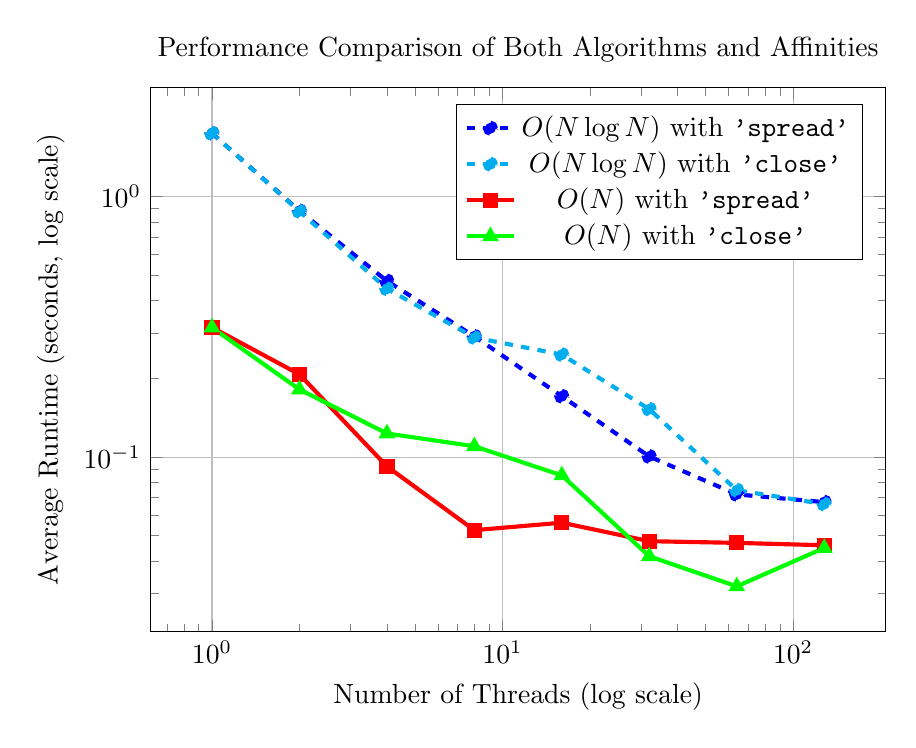
\begin{tikzpicture}
    % Define the data for all four experiments
    \pgfplotstableread[col sep=comma]{
        Threads, p1_Spread, p1_Close, p2_Spread, p2_Close
        1,       1.75128,   1.75211,  0.31491,   0.31448
        2,       0.88190,   0.87836,  0.20789,   0.18196
        4,       0.47461,   0.44315,  0.09218,   0.12330
        8,       0.29084,   0.28787,  0.05244,   0.11012
        16,      0.17135,   0.24754,  0.05603,   0.08512
        32,      0.10060,   0.15278,  0.04758,   0.04163
        64,      0.07197,   0.07469,  0.04688,   0.03192
        128,     0.06721,   0.06604,  0.04590,   0.04482
    }\alldata

    \begin{loglogaxis}[
        title={Performance Comparison of Both Algorithms and Affinities},
        xlabel={Number of Threads (log scale)},
        ylabel={Average Runtime (seconds, log scale)},
        legend pos=north east,
        grid=major,
        width=0.9\textwidth,
        height=0.7\textwidth, % Slightly taller for 4 lines
    ]
    
    % Plot p1 'spread'
    \addplot [color=blue, mark=*, line width=1.5pt, dashed] table [
        x=Threads,
        y=p1_Spread
    ] {\alldata};
    \addlegendentry{$O(N \log N)$ with \texttt{'spread'}}

    % Plot p1 'close'
    \addplot [color=cyan, mark=*, line width=1.5pt, dashed] table [
        x=Threads,
        y=p1_Close
    ] {\alldata};
    \addlegendentry{$O(N \log N)$ with \texttt{'close'}}
    
    % Plot p2 'spread'
    \addplot [color=red, mark=square*, line width=1.5pt] table [
        x=Threads,
        y=p2_Spread
    ] {\alldata};
    \addlegendentry{$O(N)$ with \texttt{'spread'}}
    
    % Plot p2 'close'
    \addplot [color=green, mark=triangle*, line width=1.5pt] table [
        x=Threads,
        y=p2_Close
    ] {\alldata};
    \addlegendentry{$O(N)$ with \texttt{'close'}}
    
    \end{loglogaxis}
    \end{tikzpicture}
    % --- End PGFPlots Figure ---
    \caption{Performance comparison of both $O(N \log N)$ (p1) and $O(N)$ (p2) algorithms using both \texttt{'spread'} and \texttt{'close'} affinity. This graph clearly shows the high overhead of the p1 algorithm and the NUMA First Touch effect for the p2 algorithm.}
    \label{fig:affinity}
\end{figure}

\begin{table}[h!]
    \centering
    \caption{Speedup of $O(N)$ Algorithm (p2): \texttt{'spread'} vs. \texttt{'close'}}
    \label{tab:speedup_affinity}
    \begin{tabular}{rcc}
        \toprule
        Threads & Speedup with \texttt{'spread'} & Speedup with \texttt{'close'} \\
        \midrule
        1   & 0.24x & 0.24x \\
        2   & 0.36x & 0.41x \\
        4   & 0.81x & 0.60x \\
        8   & \textbf{1.42x} & 0.68x \\
        16  & \textbf{1.33x} & 0.87x \\
        32  & 1.56x & \textbf{1.79x} \\
        64  & 1.59x & \textbf{2.33x} \\
        128 & \textbf{1.62x} & 1.66x \\
        \bottomrule
    \end{tabular}
\end{table}



\end{document}